\chapter{Intensidad eléctrica y fuerza electromotriz}
\chaptermark{Intensidad eléctrica y fem}

\begin{miparrafo}
La corriente eléctrica es el flujo de carga eléctrica que recorre un material. Se debe al movimiento de las cargas (normalmente electrones) en el interior del mismo. Al caudal de corriente (cantidad de carga por unidad de tiempo) se le denomina intensidad de corriente eléctrica(representada comúnmente con la letra I). En el Sistema Internacional de Unidades se expresa en culombios por segundo (C/s), unidad que se denomina ampere, A. El nombre de ampere es en honor al físico francés André-Marie Ampère (1775-1836). 

El instrumento usado para medir la intensidad de la corriente eléctrica es el galvanómetro que, calibrado en amperios, se llama amperímetro, colocado en serie con el conductor por el que circula la corriente que se desea medir.


Históricamente, la corriente eléctrica se definió como un flujo de cargas positivas (+) y se fijó el sentido convencional de circulación de la corriente, como un flujo de cargas desde el polo positivo al negativo. Sin embargo posteriormente se observó, gracias al efecto Hall, que en los metales los portadores de carga son negativos, electrones, los cuales fluyen en sentido contrario al convencional. En conclusión, el sentido convencional y el real son ciertos en tanto que los electrones como protones fluyen desde el polo negativo hasta llegar al positivo (sentido real), cosa que no contradice que dicho movimiento se inicia al lado del polo positivo donde el primer electrón se ve atraído por dicho polo creando un hueco para ser cubierto por otro electrón del siguiente átomo y así sucesivamente hasta llegar al polo negativo (sentido convencional). Es decir la corriente eléctrica es el paso de electrones desde el polo negativo al positivo comenzando dicha progresión en el polo positivo.

En el siglo XVIII cuando se hicieron los primeros experimentos con electricidad, solo se disponía de carga eléctrica generada por frotamiento (electricidad estática) o por inducción. Se logró (por primera vez, en 1800) tener un movimiento constante de carga cuando el físico italiano Alessandro Volta inventó la primera pila eléctrica.
\end{miparrafo}

\section[Corriente eléctrica. Intensidad y densidad de corriente]{Corriente eléctrica. Intensidad y densidad de corriente\sectionmark{Corriente eléctrica}}
\sectionmark{Corriente eléctrica}

Hay una ley termodinámica que asegura que un sistema de partículas que se encuentra en un medio tiene una energía cinética que vale $\frac 3 2 KT$, 	donde $k$ es la constante de Boltzman y $T$ la temperatura absoluta.

Las partículas cargadas tienen, pues, un movimiento aleatorio en el interior de una determinado material debido a la temperatura. Supongamos que a ese material le conectamos a una batería, es decir, lo sometemos a la acción de una campo eléctrico. Ahora, las partículas, además de la componente aleatoria, tendrán una componente en la dirección del campo. Este flujo de cargas es lo que se llama \emph{corriente eléctrica}, hay un flujo neto de cargas, distinto de cero, en una dirección.

La magnitud que vamos a introducir para expresar cuantitativamente la corriente eléctrica es la \emph{intensidad de corriente eléctrica}, $I$, que representa \emph{la cantidad de carga por unidad de tiempo que atraviesa la sección normal de un conductor},

\begin{equation}
I\ = \ \dv{q}{t}	
\end{equation}

En el sistema internacional se expresa en $\mathrm{C\ s}^{–1}=\mathrm{A}$, amprère,  si tomamos el $\mathrm{C}$ como unidad fundamental. 

En un conductor homogéneo e isótropo, $I=cte$, que está relacionado con la ecuación de la continuidad de la hidrodinámica. La conservación de la carga exige que la carga no se puede almacenar ni aniquilar en diversos tramos del conductor.

Ahora, las cargas en un conductor no solo podrán circular por su superficie (conductora aislado en tema anterior) sino que lo harán por todo su interior.

Necesitamos de una \emph{fuente} que nos proporcione energía para que las cargas se puedan mover:

$$\displaystyle P\ =\ \dv{W}{t}\ = \ \dv{ q \ V}{t}\ =\ I\ V$$

Por convenio, se suele definir una dirección de la corriente eléctrica y éste es el que tomarían las cargas libres positivas, aunque el la mayoría de los metales lo que ¡realmente se mueven son los electrones, cargas negativas.

Introducimos una nueva magnitud que representará la corriente eléctrica a escala diferencial, es la \emph{densidad d corriente}, $J$:

$$J\ =\ \displaystyle \dv{I}{S'}$$

La densidad de corriente es la intensidad de corriente eléctrica por unidad de sección normal del conductor.

$\vec J=J\vec u_q$, con $\vec u_q$ vector unitario en la dirección y sentido del movimiento de las supuestas cargas positivas. 

$\vec J \cdot \dd \vec S = J \dd S \cos \theta = J \dd S'$

Con esto, $\quad \displaystyle I\ = \ \int_S \vec J \dd \vec S$

En un conductor homogéneo, $J=cte \ \to I=\int J \dd S = I \int \dd S = JS \ \to \to I=cte$, independiente del tiempo.

\section{Conductividad eléctrica. Ley de Ohm}

\begin{multicols}{2}
Los dieléctricos se caracterizan por la susceptibilidad eléctrica. Introduciremos una nueva magnitud que medirá la capacidad que tienen las cargas para moverse en el interior de un conductor (metal), es la \emph{conductividad eléctrica}.

Los átomos de los metales se disponen en una estructura cristalina en que los electrones están libres.

\begin{figure}[H]
	\centering
	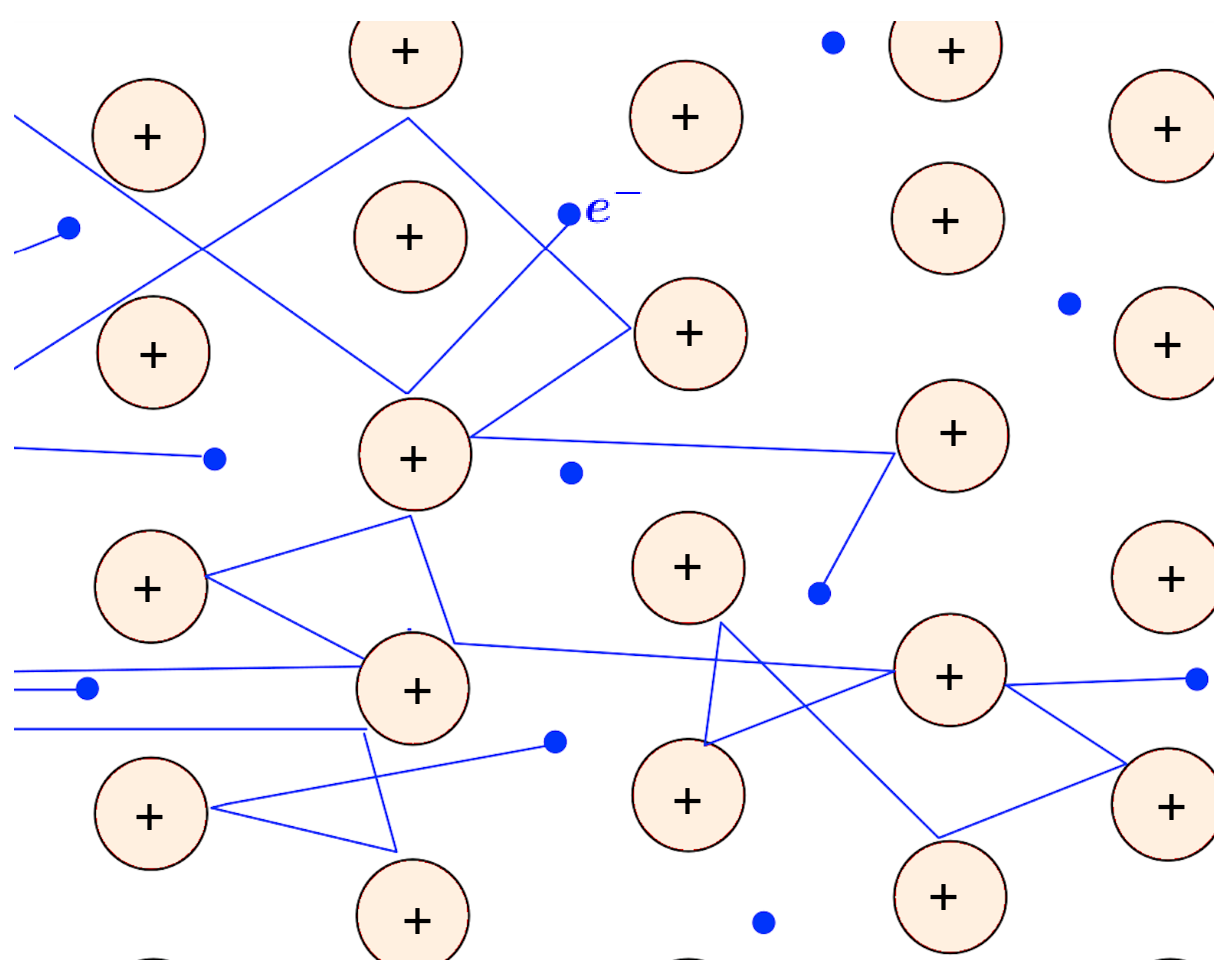
\includegraphics[width=.4\textwidth]{imagenes/imagenes25/T25IM01.png}
\end{figure}
\end{multicols}

La \emph{conductividad eléctrica} $\sigma$ mide la capacidad de moverse que tienen los electrones de moverse en la red cristalina dependiendo de lo espaciada o comprimida que esté la red, da la idea de la facilidad con que un electrón puede moverse en el interior de un metal.

El físico alemán Georg Simon Ohm (1789-1854) experimentó con muchos metales y enunció la ley experimental que lleva su nombre y dice \emph{``En un conductor, a $T$ constante, la razón entre la diferencia de potencial entre dos puntos, $V$ y la intensidad de la corriente eléctica que circula, $I$, es constante''}. A la constante de proporcionalidad, que depende de la naturaleza del conductor, se le llama \emph{\textbf{resistencia}} del metal, $R$.

\begin{equation}
\subrayado{ \ \boxed{ \ \boldsymbol{ \dfrac V I \ = \ R	} \ } \ } \qquad \textbf{Ley de Ohm}
\end{equation}

Posteriores estudios demostraron que esta ley la cumplen una gran gama de metales en una gran gama de temperaturas, la ley es casi independiente de la temperatura.

La resistencia, en el sistema internacional de unidades s expresa en $\mathrm{V \ A}^{-1}= \mathrm{\Omega}$ y recibe el nombre de Omh, en honor a su descubridor.

Considenemos un conductor metálico y cilíndrico, de longitud $l$ y vamos a calcular el campo eléctrico.

En el caso unidimensional, $\ \displaystyle E=-\dv{V}{x} \ \to \ V=E\ l$. La conductividad $\sigma$ está relacionada con la estructura cristalina del metal y con $E$.

Al estar considerando un conductor eléctrico, $I=J\ S$, tendremos

$\dfrac V I = \dfrac {E\ l}{J\ S}=R \ \to \ J=\dfrac{l}{R\ S} \ E$

$\dfrac{l}{R\ S}$ depende de las características geométricas y de la naturaleza del metal y $E$ es la magnitud aplicada, así, llamamos

$$\sigma \ = \ \dfrac {l}{R\ S} \qquad \text{conductividad eléctrica del metal} \quad \to \quad J \ = \ \sigma \ E$$

$\text{En forma vectorial: } \qquad \vec J \ = \ \sigma \ \vec E$

Vamos a interpretar la ley de Ohm dede el punto de vista dinámico o microscópico. Partimos de la ecuación de movimiento de una carga, lo aplicamos para todas las cargas y comparamos con la ley de Ohm.

$\displaystyle I=\dv{q}{t}=\dfrac{e\ \dd N}{\dd t}$, $e$ es el valor absoluto de la carga. $\ \vec J =\sigma \vec E$

Supongamos que tenemos un conductor homogéneo, con las mismas propiedades físicas en cada uno de sus puntos,

$\displaystyle J=\dfrac I S = \dfrac {e\dd N}{S \dd t}=\textcolor{gris}{\left( v=\dv{l}{t} \right)}=\dfrac{e\ dd N}{S \dd l}v=n\ e\ v$

donde $n=\dfrac{\dd N}{S \dd l}=\dfrac{\dd N}{\dd \tau}$

Vectorialmente, $\quad \vec J \ = \ n\ e\ \vec v_E$, con $\vec v_E$ la velocidad de la carga debida al campo eléctrico.

Cuando la conducción es debida a los electrones, carga negativa, tenemos:

$\vec J = -ne\vec v_E$, que comparando con $\vec J=\sigma \vec E$, se obtiene:

$\vec v_E=-\dfrac{\sigma}{n e} \vec E$, velocidad de arrastre debida al campo eléctrico.

Debido a la homogeneidad del conductor (cilíndrico en este caso), el campo eléctrico $\vec E$ por lo general va a ser constante. $\sigma$ depende de las características físicas del conductor, $n$ es la densidad de partículas y $e$ la carga de éstas. Hemos obtenido que $\vec v_E$ es constante, es la velocidad límite de arrastre. Esto significa que el electrón rozará con el resto del metal de tal manera que alcanzará la velocidad límite de arrastre.

La ecuación dinámica del electrón cuando se somete el metal a un campo eléctrico $\vec E$ es
$\ \displaystyle m \dv{\vec v}{t}=-e\vec E-k\vec v.\ $ $k$ es una constante de rozamiento (como la fuerza de Stookes) que engloba la facilidad con que el electrón puede entrar en la red cristalina.

Para que exista una velocidad límite, la aceleración ha de ser cero, por lo que $\ \displaystyle m \dv{\vec v}{t}=0 \ \to \ -e\vec E-k\vec v_E=0 \to \vec v_E=\dfrac{-e\vec E}{k}$

Comparando con la velocidad límite encontrada anteriormente, 

$\dfrac{\sigma n}{e}=\dfrac e k \ \to \ k=\dfrac{ne^2}{\sigma}$

Vamos a ampliar el problema introduciendo el \emph{tiempo de relajamiento}: es el tiempo que pasa desde que la velocidad del electrón es la de arrastre hasta que sea la de arrastre dividida por el número $e$, una vez quitado el campo eléctrico exterior· $\ t_R:\ \vec v_E \ \to \ \dfrac{\vec v_E}{e}$

Al quitar el campo, $\displaystyle m\dv{\vec v}{t}=-k\vec v \ †o \ \dv{\vec v}{\vec v}=-\dfrac m n \dd t$

$\ln v_x=-\dfrac k m t + \ln \mathcal C;\quad t=t_0:\ v_x=v_{Ex} \quad v_x=v_{Ex}e^{-kt/m}$

$\displaystyle \dv{\vec v}{\vec v}=-\dfrac m n \dd t \quad \to \quad \vec v=\vec v_E e^{-kt/m}$

Cuando $\ t=t_R \ \leftrightarrow \ \vec v=\vec v_E e^{-1}=\vec v_E e^{-kt_R/m}$

De donde, $\ t_R=m/k$, que comparando con $\ k=\dfrac{ne^2}{\sigma}$, tenemos

$$t_R \ = \ \dfrac m k \ = \ \dfrac {m\ \sigma}{n\ e^2}$$

$\sigma= l/(RS)$; $\sigma$ se puede determinar experimentalmente mediante la ley de Ohm. Para la mayoría de metales, $\sigma \sim 10^7 \ \Omega^{-1} \mathrm{m}^{-1}$

Si de la expresión $t_R  =  (m\sigma)/(n e^2)$ deducimos que $\sigma \sim 10^7 \ \Omega^{-1} \mathrm{m}^{-1}$, todo el razonamiento anterior será correcto.

\emph{Hipótesis:} Para cada electrón, hay un átomo relacionado con él.  $\ n$ número de partículas por unidad de volumen. Supongamos que cada uno de los átomos del metal contribuye como máximo con $1 \ e^{-}$, así, $\ n$ representará el número de átomos por unidad de volumen. A partir de la densidad del metal y de su número atómico podemos calcular $\ n \sim 10^{28} \ e^-/\mathrm{m}^3$.

Nos falta una estimación para el tiempo de relajamiento. El $e^-$ se mueve en una red cristalina. El $t_R$ será del órden en que el electrón tarda en interaccionar con dos átomos distintos (esto constituye otra \emph{hipótesis}).

Como $\mathcal E_c=\dfrac 3 2 k T = \dfrac 1 2 m v^2$ y la distancia entre átomos en la red cristalina es del orden de $l \sim 5\times 10^{-9}\ \mathrm{m}$ y $t\sim l/v$ tendremos $t_R \sim 10^{-14} \ \mathrm{s}$.

De ello, $t_R  =  (m\sigma)/(n e^2)$ despejamo $\ \sigma \sim 10^7 \ \Omega^{-1} \mathrm{m}^{-1}$, lo que coincide con lo encontrado experimentalmente con la ley de Ohm.

\section{Efecto Joule}

Para que el electrón se mueva, hay que aplicarle una determinada energía.  El electrón roza constantemente con la red cristalina, incluso los átomos de la red van a vibrar más, una mayor agitación térmica significa mayor energía. A medida que se mueve la red cristalina puede aportar energía al exterior: \emph{radiación electromagnética}.

\emph{La radiación electromagnética} en los metales (infrarrojo o visible, calor) se produce cuando por ellos circula una corriente eléctrica.

$P=\vec F \cdot \vec v_E=e\vec E \cdot \vec v_E$ es la potencia necesaria para acelerar un electrón  a la velocidad de arrastre.

Vamos a calcular la potencia total que se puede emitir al exterior.

La potencia por unidad de volumen, $P_\tau=-ne\vec E \cdot \vec v_E$

$P=P_\tau (SL)=--ne\vec E \cdot \vec v_E Sl=neEv_EJl =(JS)(El)=IV$

Para los conductores que cumplen la ley de Ohm, $IR=V$, tenemos

\begin{equation}
P \ = \ I \ V \ = \ I^2\ R
\end{equation}

Esquemáticamente, la resistencia en un circuito se representa por --/|/|/\---.

\section{Combinación de resistencias}

\subsection{Combinación de resistencias en serie}

\begin{figure}[H]
	\centering
	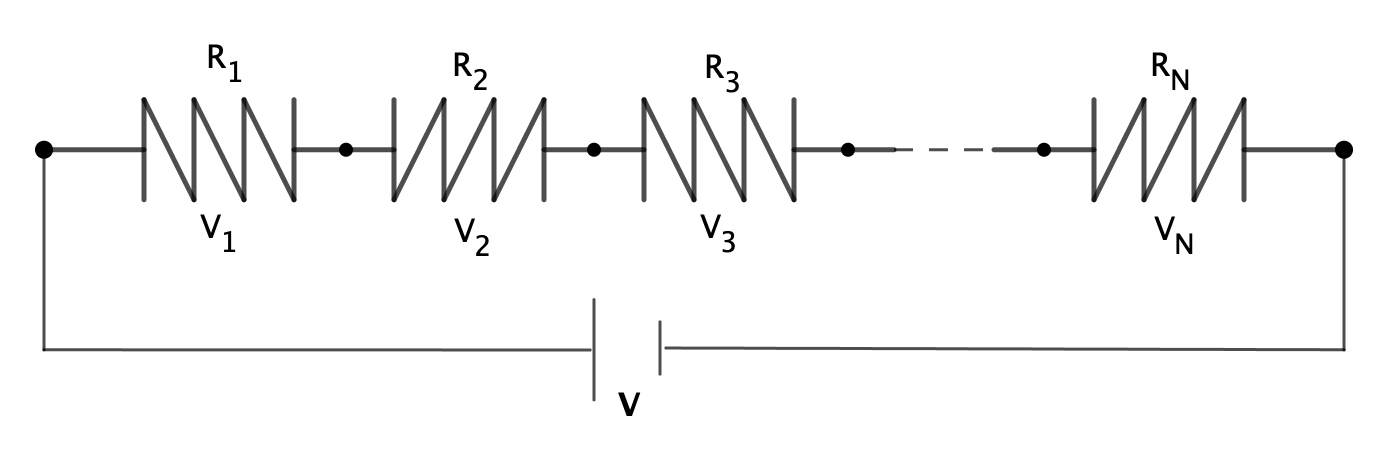
\includegraphics[width=.9\textwidth]{imagenes/imagenes25/T25IM02.png}
\end{figure}

$V=V_1+V_2+V_3+\dots +V_N;\quad I$ es la misma en todas las $R_i$

Si todos los conductores obedecen la ley de Ohm,

$V=\sum V_i= IR_1+IR_2+\cdots +IR_N=I(R_1+R_2+\cdots +R_N)$, por lo que

\begin{equation}
\boldsymbol{ R_{serie} \ = \ R_1 \ + \ R_2 \ + \ \cdots \ + \ R_N	 \ = \ \sum_{i=1}^N R_i }
\end{equation}

\subsection{Combinación de resistencias en paralelo}

Todas las resistencias están conectadas a la misma $V$, pero son atravesadas por las distintas intensidades en que se divide la intensidad total.

\begin{figure}[H]
	\centering
	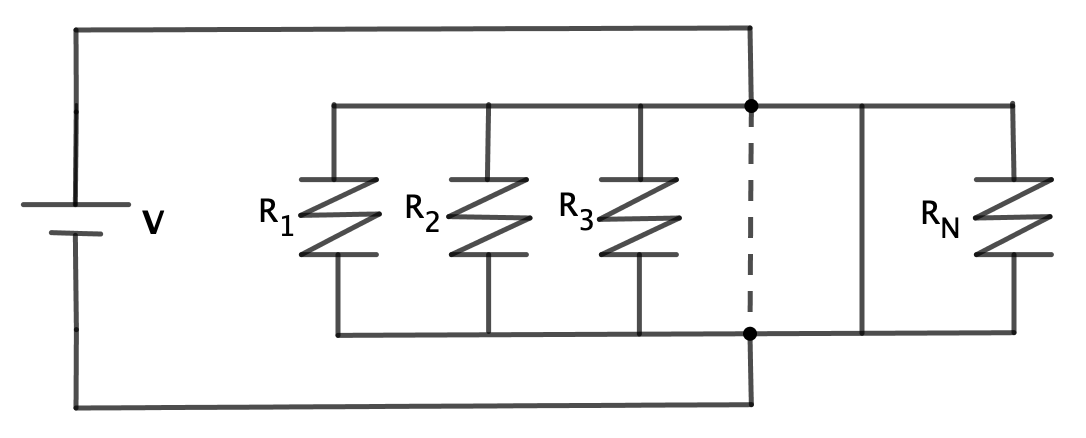
\includegraphics[width=.9\textwidth]{imagenes/imagenes25/T25IM03.png}
\end{figure}


$I=I_1+I_2+\cdots + I_N=\dfrac V{R_1}+\dfrac V{R_2}+\cdots +\dfrac V{R_N}= $

$=V \left( \dfrac 1{R_1}+ \dfrac 1{R_2}+ \cdots +\dfrac 1{R_N} \right)  =\dfrac V R$

\begin{equation}
\boldsymbol{ \dfrac 1 {R_{paralelo}} \ = \ \dfrac 1{R_1} \ + \ \dfrac 1{R_2} \ + \cdots \ + \ \dfrac 1{R_N} = \sum_{i=1}^N \dfrac 1{R_i} }
\end{equation}


\vspace{10mm} %******************************************

\begin{figure}[H]
	\centering
	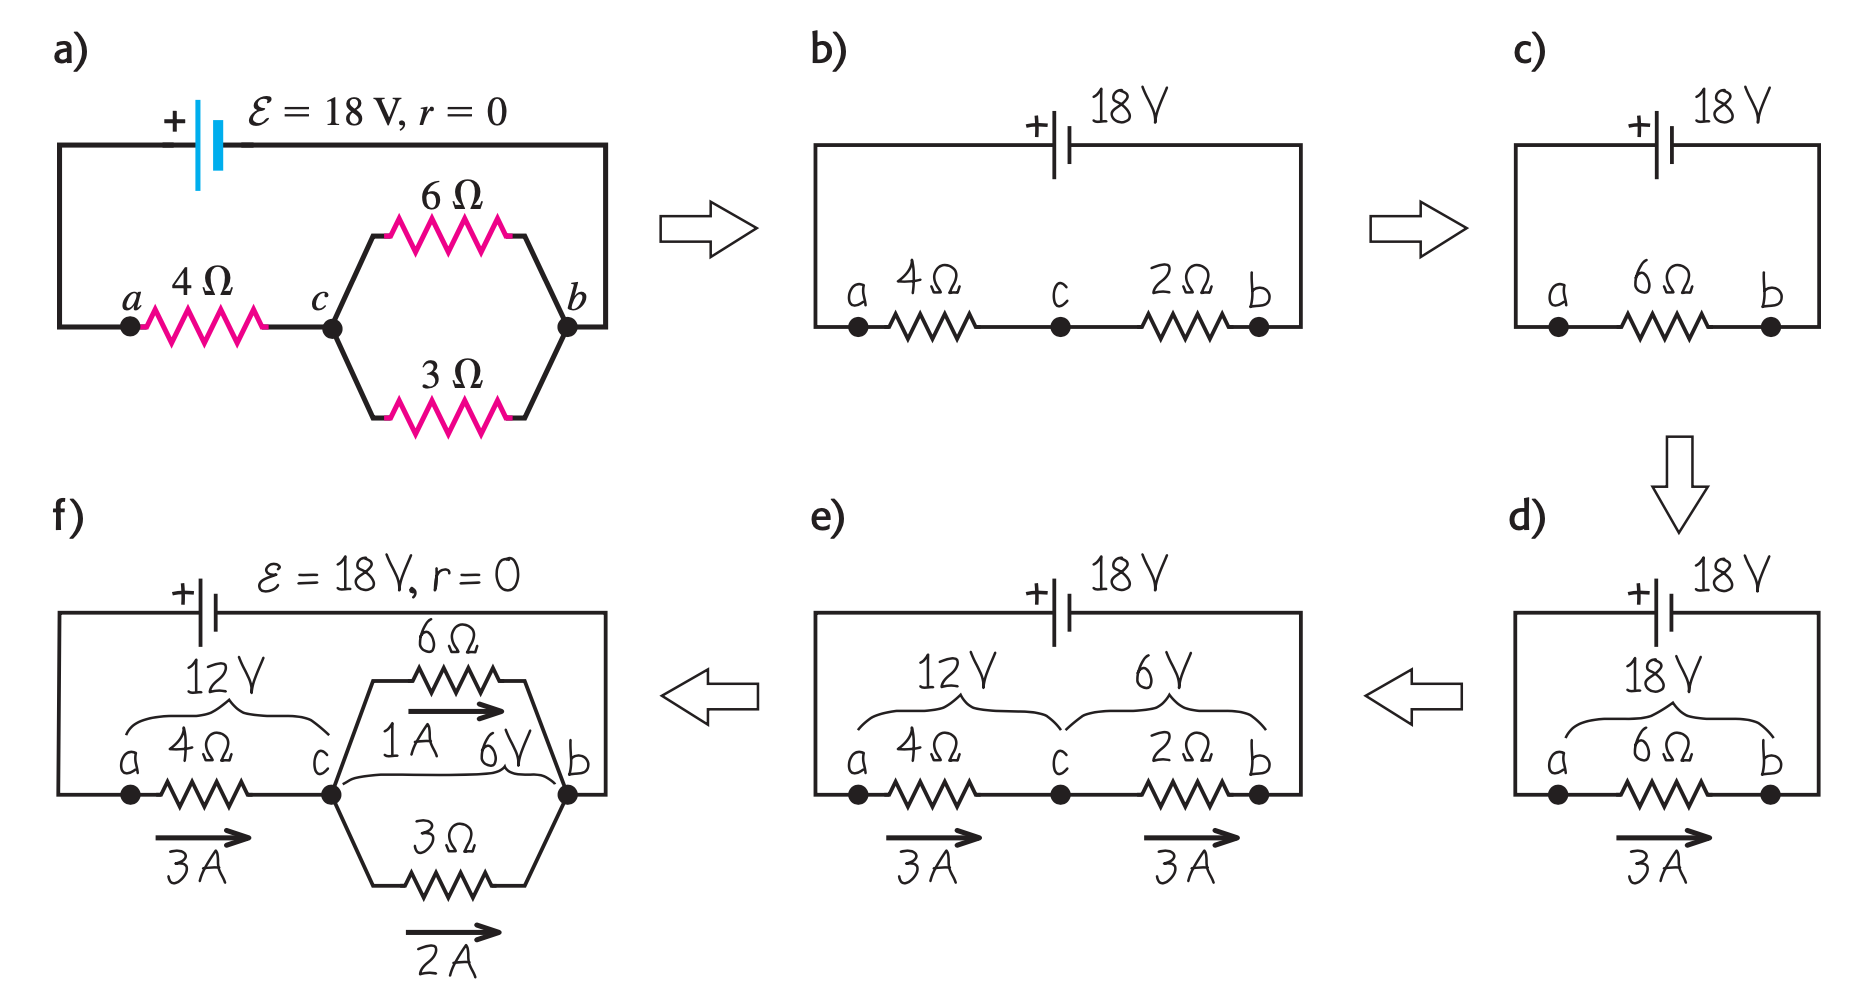
\includegraphics[width=1.05\textwidth]{imagenes/imagenes25/T25IM04.png}
\end{figure}

\section{Fuerza electromotriz}


La fuerza electromotriz (representado fem o $\varepsilon$)
es toda causa capaz de mantener una diferencia de potencial entre dos puntos de un circuito abierto o de producir una corriente eléctrica en un circuito cerrado. Es una característica de cada generador eléctrico.

El trabajo por unidad de carga que se ha de realizar para que una carga de una vuelta a un circuito es
$\ \textcolor{gris}{\left( \vec E = \dfrac {\vec F}{q} \right)} \qquad \displaystyle
\oint_C \vec E \cdot \dd \vec l = \varepsilon,\ $ \emph{fem}.

Como $\vec E$ es conservativo, $\ \displaystyle \int_1^2 \vec E \cdot \dd \vec l = V_2-V_1=V=IR$

donde, por hipótesis, hemos supuesto que el conductor es óhmico (verifica la ley de Ohm)

En campos conservativos, $\ \displaystyle \oint \vec E \cdot \dd \vec l =0 \ \to \ I=0$, en un conductor cerrado en campo conservativo no circula corriente eléctrica. Nunca podremos construir corriente eléctrica si el campo es conservativo o estacionario.

Para ello se construyen los \emph{generadores}, son capaces de ceder energía a los electrones del circuito para que se muevan en un sentido o en otro. Esta energía, por efecto Joule, desprenderá calor. Los generadores obtinen su energía de reacciones químicas (pilas Volta) o por induccción magnética.

Si el conductor es óhmico, $\varepsilon=IR$, en el $SI$ se mide en $\mathrm{V}$.

\begin{multicols}{2}
Esquema de circuito eléctrico (en corriente continua).

$R_i$ es la resistencia interna del propio generador.

$\varepsilon=I(R+R_i)$

$\varepsilon=IR_e+IR_i=V_A-V_B+IR_i$
	\begin{figure}[H]
	\centering
	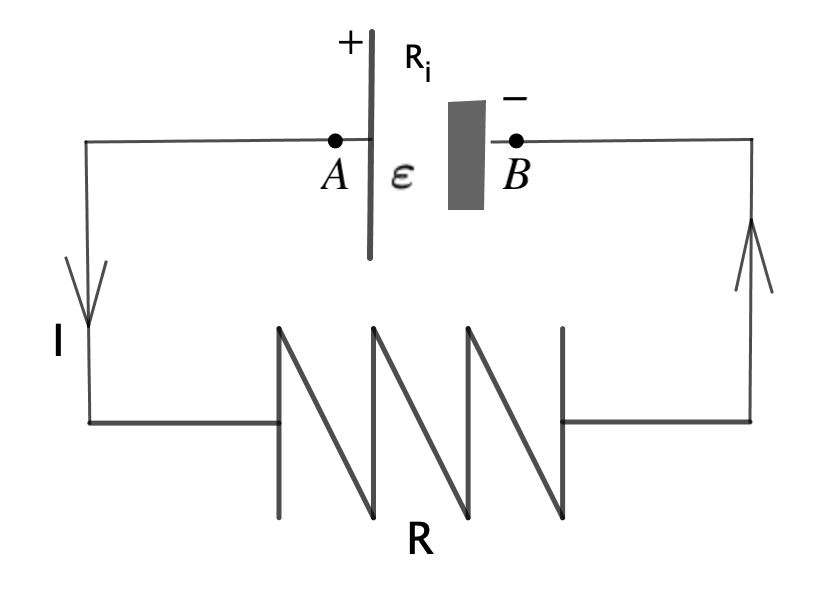
\includegraphics[width=.4\textwidth]{imagenes/imagenes25/T25IM05.png}
\end{figure}
\end{multicols}
$V_A-V_B$ es la diferencial de potencial a que se conecta la resistencia externa, tiene lugar en el interior del generador.

Por ello, $ \ \varepsilon > V$

Cuando se conecta un motor $G'$ a un generador $G$, aplicando el teorema de conservación de la energía, tenemos

$\varepsilon I=I^2(R+R_i+r_i)+\varepsilon' I \ \to \ I=\dfrac{\varepsilon -\varepsilon'}{R+R_i+r_i}= \dfrac{\sum_i \varepsilon_i}{\sum_i R_i}$

donde $r_i$ representa la resistencia interna del motor o paratos conectados y $\varepsilon'$ es la \emph{fuerza contra electromotriz}.

\section{Leyes de Kirchoff. Redes eléctricas}

\begin{multicols}{2}
Una \emph{red} eléctrica no es más que una combinación de fem y fcem (fuerza electromotriz y contra electromotriz).

Un \emph{nudo} eléctrico es la región donde confluyen dos o más conductores.
	\begin{figure}[H]
	\centering
	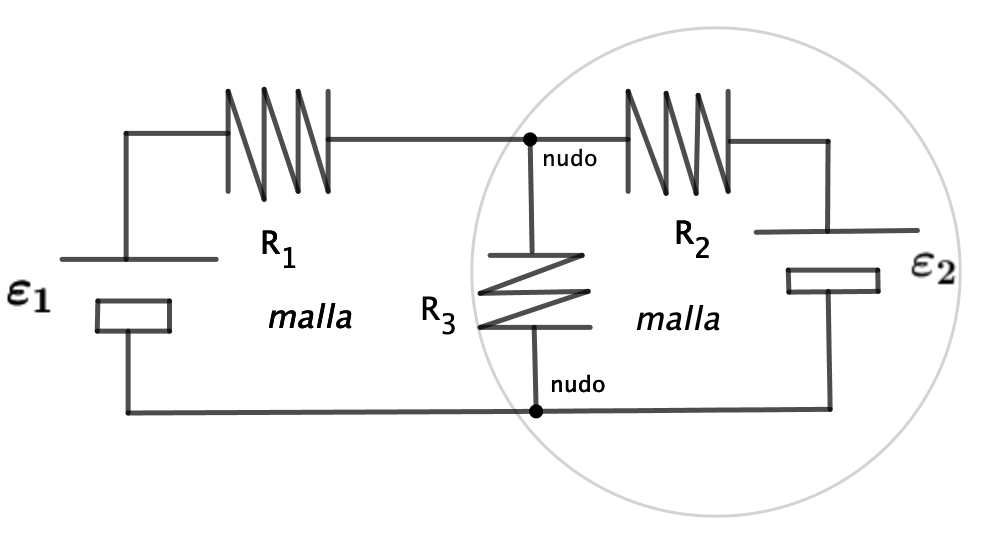
\includegraphics[width=.5\textwidth]{imagenes/imagenes25/T25IM07.png}
\end{figure}
\end{multicols}
Se asignan llas intensidades que van a ciercular por cafa rama y se aplican las \colorbox{LightYellow}{ \emph{\textbf{leyes de Kirchoff}} }. Se basan en dos teoremas de conservación: el teorema de conservación de la carga y el teorema de conservación de la energía.

\begin{miparrafodestacado}
\begin{enumerate}
	\item En cualquier nudo de la red, la suma de las intensidades ha de ser cero.
	\item La suma de las caídas de potencial a lo largo de cualquier camino cerrado en una red es nula.
\end{enumerate}
\end{miparrafodestacado}

Analicemos la sigiuiente red red donde aparecen 3 corrientes de rama.

\begin{multicols}{2}
Se elige, arbitrariamente,  un sentido de recorrido de malla.

Se toman como positivas las intensidades que salen del nudo y negativas la que entran. Aplicando la $1^a$ de Kirchoff al nudo superior de la imagen:
	\begin{figure}[H]
	\centering
	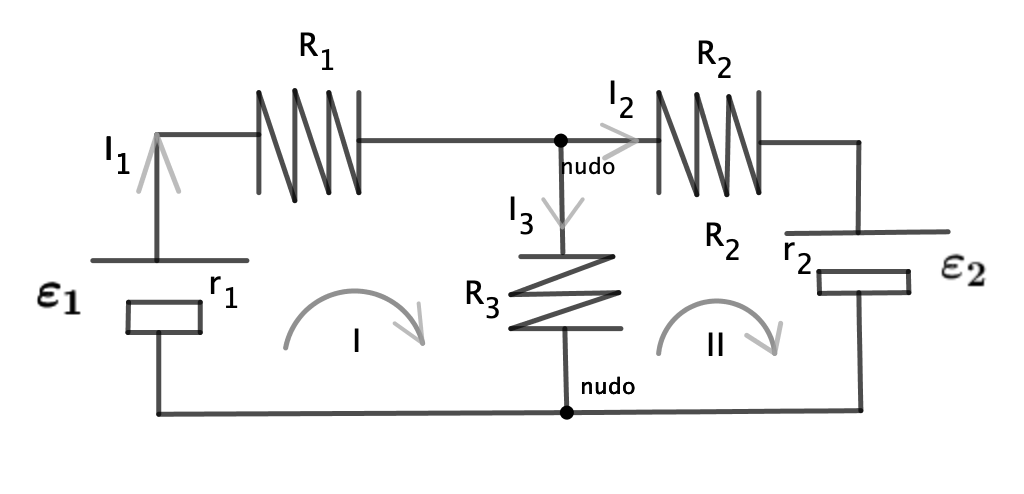
\includegraphics[width=.55\textwidth]{imagenes/imagenes25/T25IM08.png}
\end{figure}
\end{multicols}
$-I1+I_2+I_3=0$

En cuanto a la segunda ley:

\begin{itemize}
\item El sentido de las fem es el siguiente, si el sentido que hemos elegido de malla hace que la `corriente de malla' entre por el borne negativo y salga por el postivo, la femm es positiva; en caso contrario la tomaremos negariva. En la figura anterior, $\varepsilon_1>0,\ \varepsilon_2<0$

\item El sentido de las caídas de tensión en las resistencias será positivo si la intensidad que la atraviesa lleva el mismo sentido que la `corriente de malla' y negativo en caso contrario. Así, tendremos $+I_1R_1; \ +I_2 R_2; \ -I_3R_3$ en la malla II. 
\end{itemize}

\vspace{5mm} %************************************
\begin{miparrafodestacado}
	Plantearemos la primera ley de Kirchoff a $n-1$ nodos de la red y completaremos las ecuaciones necesarias aplicando la segunda ley de kirchoff a las mallas que haga falta.
\end{miparrafodestacado}

$$ \begin{cases}
 \ \text{nudo superior} & -I_1+I_2+I_3=0 \\
 \ \text{malla I} & -\varepsilon_1+I_1(R_1+r_1)+I_3R_3=0 \\
 \ \text{Malla II} & +\varepsilon_2+I_2(R_2+r_2)-I_3R_3=0
 \end{cases}$$
 
 Tenemos 3 ecuaciones con 3 incógnitas, $I_1,\ I_2,\ I_3$.
 

 
 \begin{multicols}{2}
En los circuitos sencillos solo hay una malla y ningún nodo.

 $$\varepsilon - I(R+R_1)=0$$
 
 $\quad$
	\begin{figure}[H]
	\centering
	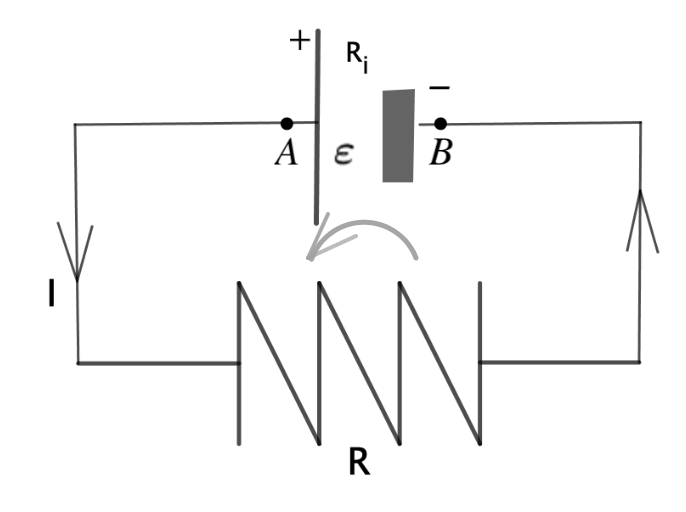
\includegraphics[width=.3\textwidth]{imagenes/imagenes25/T25IM09.png}
\end{figure}
\end{multicols}
 
 \section{Problemas}

\begin{prob}
Demostrar que si en una bateria de fem fija $\varepsilon$ y resistencia interna $r_i$ se conecta a una resistencia exterior $R$, se suministra máxima energía a la resistencia exterior cuando $R=r_i$	
\end{prob}

$\varepsilon I=I^2R+I^2r_i;\quad P_{ext}=I^2R \ \to \ P_{ext}=\varepsilon I-I^2 r_i$

Ohm: $\ \varepsilon =I(R+r_i) \to I=\dfrac{\varepsilon}{R+r_i}$, con lo que

$P_{ext}=\dfrac{\varepsilon^2}{R+r_i}-\dfrac{\varepsilon^2}{(R+r_i)^2}Rî=\dfrac{\varepsilon^2}{(R+r_i)^2} \ [(R+r_i)-r_i]=\dfrac{\varepsilon^2 R}{(R+r_i)^2}$

$\varepsilon,\ r_i$ son datos, por lo que $\ P_{ext}=P_{ext}(R)$

máximo cuando $\ \displaystyle \dv{P_{ext}}{R}=0:$

$\displaystyle \dv{P_{ext}}{R}=\dfrac{\varepsilon^2(R+r_i)^2-\varepsilon R 2(r+r_i)}{(R+r_i)^4}=\dfrac{\varepsilon^2}{(R+r_i)^4} [ (R+r_i)^2-2R^2-2Rr_i ]=\dfrac{\varepsilon^2}{(R+r_i)^4} [-R^2-r_i^2]=0 \leftrightarrow R^2= r_i^2 \ \Rightarrow \ R=r_i$


\begin{prob}
Calcula las corrientes de rama en los circuitos de las figuras adjuntas y averigua la ddp entre los puntos A y B	
\end{prob}

\begin{figure}[H]
	\centering
	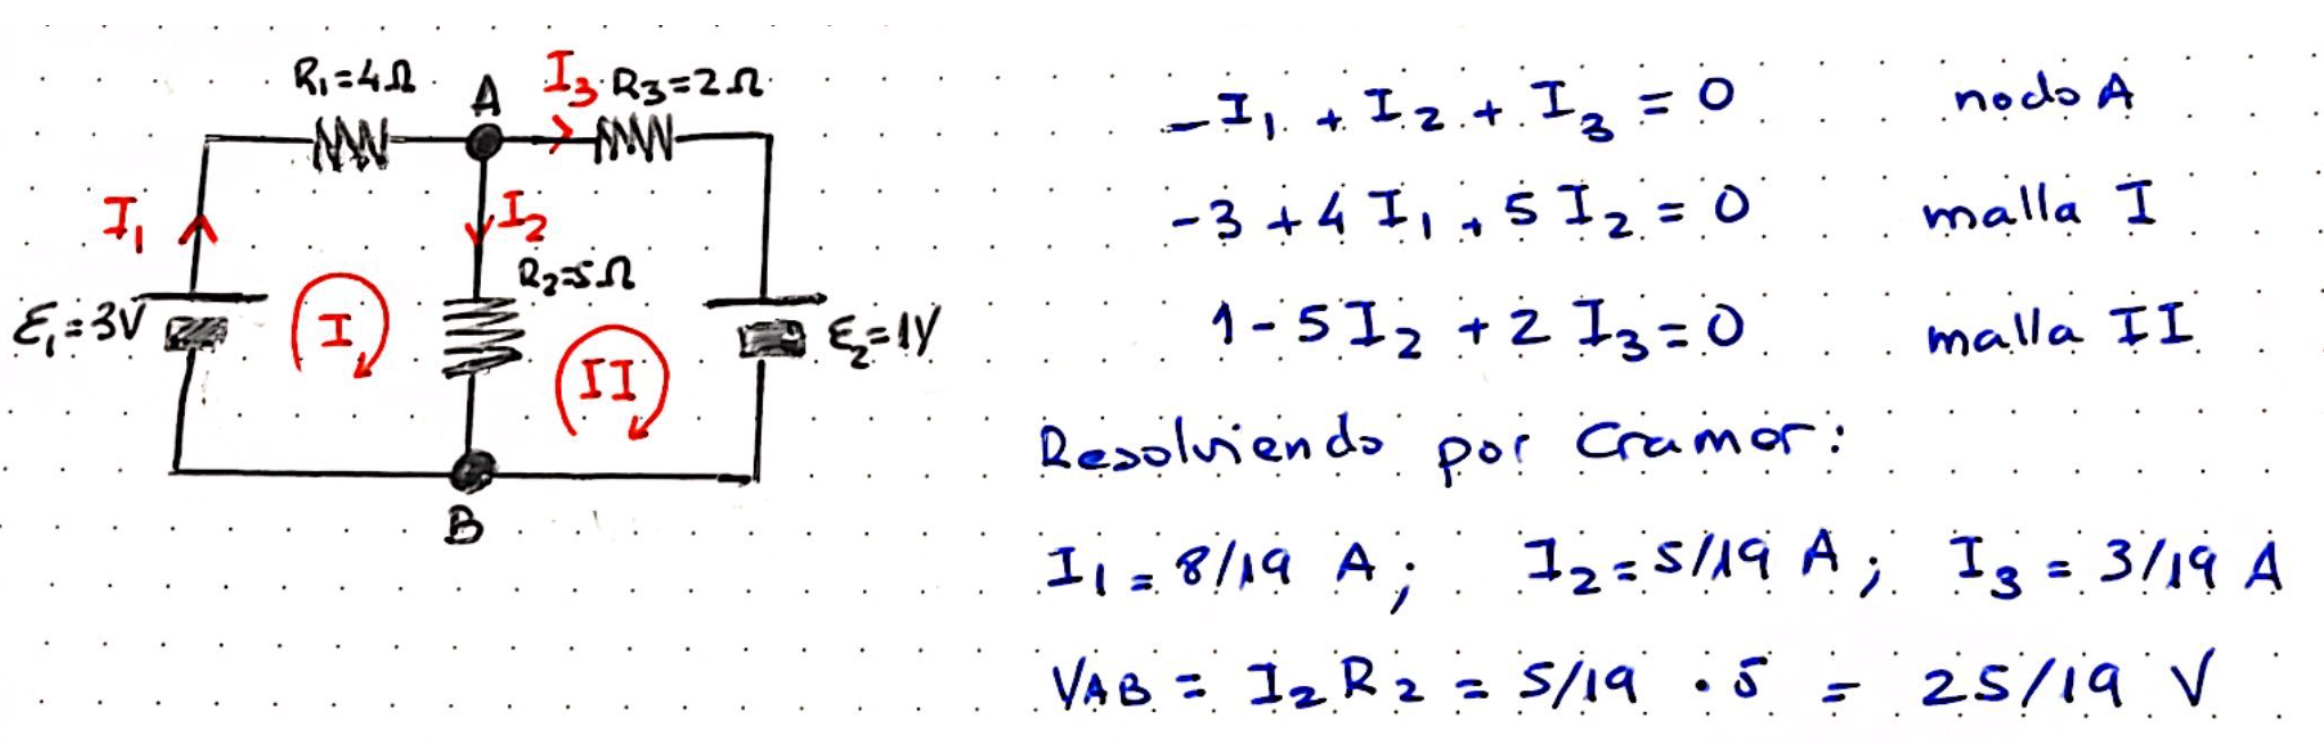
\includegraphics[width=1\textwidth]{imagenes/imagenes25/T25IM10.png}
\end{figure}

\begin{figure}[H]
	\centering
	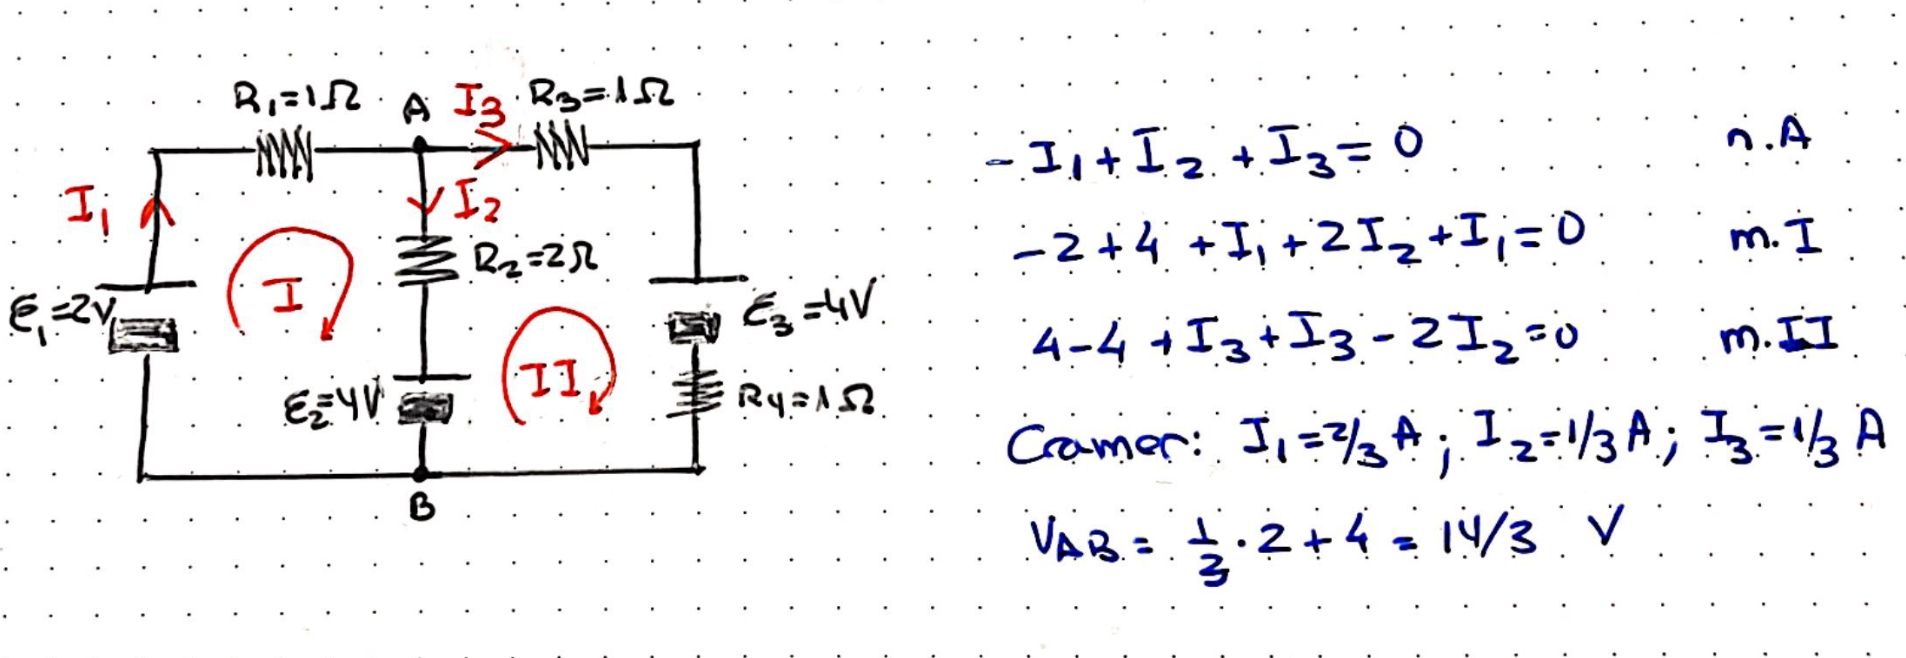
\includegraphics[width=1\textwidth]{imagenes/imagenes25/T25IM11.png}
\end{figure}


\begin{prob}
Se desea convertir un galvanómetro con $r_i=20\ \Omega$ que puede medir hasta $I_a=1\ \mathrm{mV}$ en

a) un amperímetro que pueda medir intensidades de $I=20\ \mathrm{mA}$

b) un voltímetro que pueda medir ddp de hasta $V=10\ \mathrm{V}$
\end{prob}

Los amperímetros se conectan en serie al circuito y los voltímetros en paralelo.

--- a) Al conectarle al amperímetro una resistencia externa $R$ en paralelo y montar el sitema en serie en  la rama del circuito cuya $I=2\times 10^{-2} \ \mathrm{A}$ que deseamos medir, ambas ramas, las del amperímetro y las de la resistencia externa, son atravesadas por intensidades $I_1 \text{ y } I_R$ tales que $I=I_a+I_R$

Al estar en paralelo en el circuito, ambas están conectadas a la misma ddp:

$I_a r_i =(I-I_a) R \ \to \ R=\dfrac{I_a r_i}{I-I_a}=\dfrac{10^{-3} \cdot 20}{5\times 10^{-2}-10^{-3}}=0.408\ \Omega$

--- b) Para que el galvanómetro anterior, que  mide una ddp $V=I r = 0.02 \ \mathrm{V}$ pueda medir mayores voltajes se le añade una resistencia $R$ en serie y se conecta el sistema en paralelo a los extremos del circuito donde se desea medir la $V=10\ \mathrm{V}$

La intensidad que atraviesa la resistencia interna del aparato y la externa en serie añadida es la misma y ha de ser la que puede soportar el aparato, $I=10^{-3} \ \mathrm{A}$ 

Como El potencial que se desea medir es de $V=20 \ \mathrm{V}$, lo intercalamos en paralelo al circuito y tendremos que

$V=I(R+r_i) \ \to \ R=\dfrac V I - r_i = \dfrac{10}{10^{-3}}-20=9980\ \Omega$


\newpage %*********************************************


\begin{myblock}{Esquemas circuito eléctrico (continua)}
	\begin{figure}[H]
	\centering
	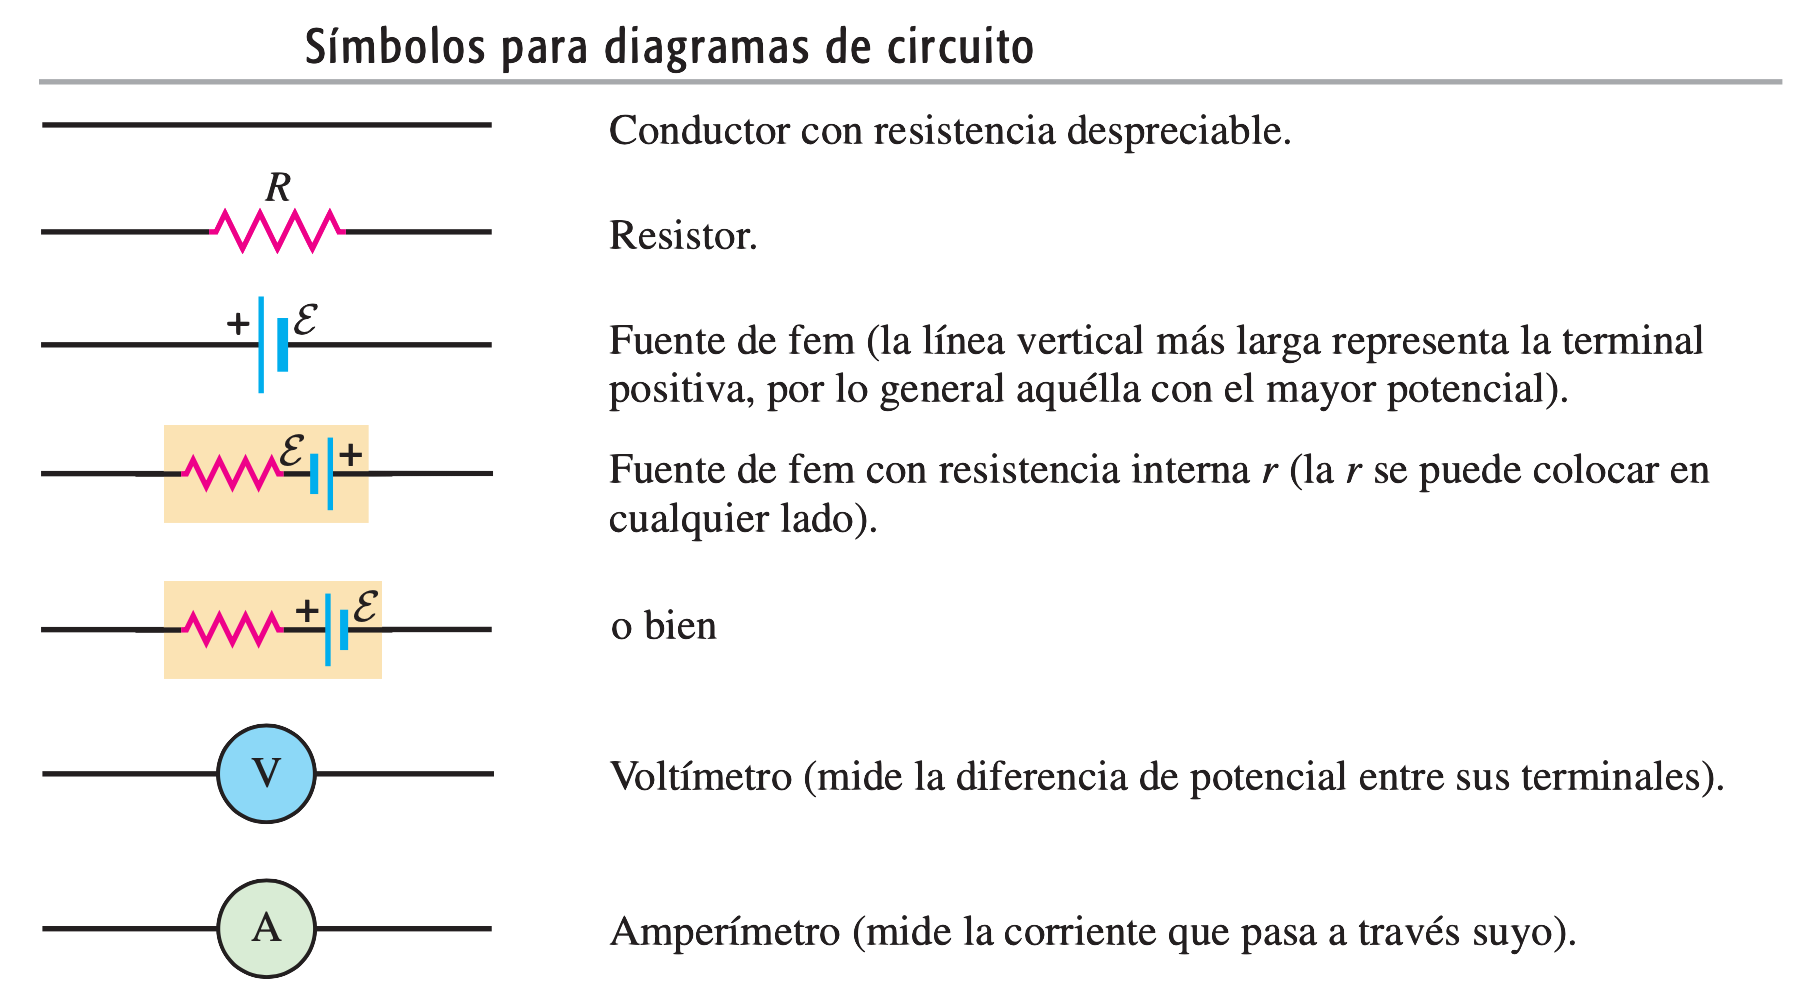
\includegraphics[width=1\textwidth]{imagenes/imagenes25/T25IM06.png}
\end{figure}	
\end{myblock}






